\chapter{The limit of a network}
\label{ch:graphons}

\section{A photograph of the whole}

The last chapter counted communities. It found that the number grows as a power
of the size, $B\propto n^{\beta}$ with $\beta\approx0.61$, and compared that
exponent with the $\sqrt{n}$ of the self-similar models. This chapter asks what
that comparison means, and the answer turns out to reach further than the
question.

Start with a way of looking at a network that we have not used yet. Draw its
adjacency matrix as a picture: one pixel for each pair of nodes, black if they
are linked, white if they are not. Order the nodes so that similar ones sit
together. Now grow the network and watch the picture. If the network is
\emph{dense} --- if each node links to a fixed \emph{fraction} of the others ---
the picture settles down. The individual pixels become too small to see, and what
survives is a pattern of greys: a smooth function $W(x,y)$ on the unit square
giving, for each pair of positions, the probability of a link
(Figure~\ref{fig:gr-limit}a). That limiting function is called a \emph{graphon},
and it is the object that a growing dense network converges to
\citep{lovasz2006,borgs2008}. Two networks with the same graphon are the same
network as far as any large-scale statistic can tell.

\begin{figure}[t]
\centering
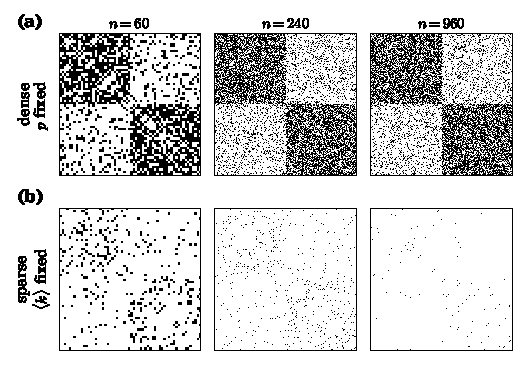
\includegraphics[width=\linewidth]{figs/fig-gr-limit.pdf}
\caption{\textbf{The limit picture, under two scalings.} Adjacency matrices of the
same two-block structure at $n=60$, $240$, $960$, nodes ordered by block.
(a)~Dense: the link probabilities are held fixed, and the picture sharpens onto a
step function --- the graphon. (b)~Sparse: the mean degree is held fixed instead,
so the probabilities fall as $1/n$. The structure is identical, and just as
detectable, but the picture fades to white. Real networks are of the second kind.}
\label{fig:gr-limit}
\end{figure}

This is a powerful idea, and it has a large and beautiful theory attached to it.
It is also, applied naively to the networks in this book, useless --- and the
precise way in which it fails is instructive. The reason is the second row of
Figure~\ref{fig:gr-limit}. Real networks are not dense. The Internet, the
interactome, a co-authorship graph, all keep a roughly fixed mean degree as they
grow; so does every model in this book. When the mean degree is fixed the link
probability falls like $1/n$, the pixels thin out, and the picture converges ---
to white. The limit exists, and it has thrown away everything we care about.

The obvious repair is to turn up the contrast: divide the whole picture by its
own average darkness before taking the limit, so that what survives is the
\emph{pattern} of the greys rather than their absolute level. This works, and it
is the substance of a theory of sparse graph limits developed by
\citet{borgs2019}. Rescaling costs something --- the rescaled function is no
longer a probability bounded by one, so the limit object is no longer a bounded
function but an $L^p$ one, and the theory must be rebuilt around that --- but the
gain is real. It is the first limit theory that copes with hubs, and with the
power-law degree distributions that come with them.

There are then three regimes, not two, and it is worth knowing which one a
network is in. Dense networks have ordinary bounded graphons. Networks that are
sparse but \emph{densifying} --- the link probability falling to zero while the
mean degree still creeps up --- have $L^p$ graphons. And networks of genuinely
fixed mean degree have neither. The rescaling that saves the middle case needs the
mean degree to grow without bound, and when it does not, the rescaled picture
concentrates instead of settling: for the ring it piles up along the diagonal,
approaching not a function but a line of infinite density.

Which regime a real system is in is a question with an answer, and the systems
followed through this book do not give the same one. Track the mean degree against
size and fit $\langle k\rangle\propto n^{\delta}$: the Internet at the
autonomous-system level, over $733$ snapshots, gives $\delta=-0.04$ --- flat, or
very slightly thinning, a mean degree that stays near four while the network grows
sixty-fold. That is the third regime, and no limit theory yet reaches it. The
cond-mat co-authorship network gives $\delta=+0.36$, and its mean degree climbs
from $2.2$ to $19$ as it grows from four hundred to four hundred thousand authors.
That is the middle regime: co-authorship densifies, and it is the one system here
that the $L^p$ theory actually covers.

The interactomes appear to densify too, more gently, but the appearance should not
be trusted: that series runs across \emph{organisms} rather than across time, and
a better-studied organism has both more proteins catalogued and more interactions
recorded per protein. The trend there measures the attention of biologists at
least as much as the architecture of cells.

Even the middle regime is tighter than it looks, in a way the book's own models
can measure. Membership in $L^p$ is a condition on how extreme the hubs are: for a
degree distribution $p(k)\sim k^{-\gamma}$ it holds when $p<\gamma-1$, and the
theory needs $p>1$, so there is a usable window only for $\gamma>2$. The
pseudofractal web of the last chapter has $\gamma\simeq2.585$, leaving the window
$1<p<1.585$; real networks, whose exponents cluster between two and three, are all
squeezed into the same narrow slot, and it closes entirely as $\gamma\to2$. The
limit theory reaches the scale-free world, but only just.

Being in the third regime is worth stating plainly, because it explains the shape
of the previous chapter. The evidence for a partition there grew like $m\ln K$, in
proportion to the number of \emph{links}; the graphon limit normalizes by the
number of \emph{pairs}, which is $n^2$. The two scales differ by the mean degree, and in
the sparse world that ratio is the whole story. It is why the last chapter had to
compute at finite $n$ and could not simply take a limit. The finite-size
calculation was not a convenience. It was the only instrument that sees anything.

\section{The block model was a graphon all along}
\label{sec:gr-blockmodel}

Set the difficulty aside for a moment, because the language is useful even where
the limit theorem is not.

A stochastic block model \emph{is} a graphon --- the simplest interesting kind. If
the nodes fall into blocks and the link probability depends only on which blocks
the endpoints are in, then $W$ is a step function: constant on each rectangle,
jumping at the block boundaries. Fitting a block model to a network is fitting a
step function to a picture, and asking how many blocks it needs is asking how
finely the picture must be pixelated before the description stops improving.

The degree-corrected model of the last chapter is a graphon too, and its shape
says exactly what degree correction \emph{does}.

\begin{calculation}{degree correction, as a factorization}
Let the graphon factorize as
\begin{equation}
  W(x,y) = f(x)\,f(y)\;w\big(g(x),g(y)\big),
  \label{eq:gr-factor}
\end{equation}
where $g(x)$ names the block at position $x$, $w$ is constant on block pairs, and
$f$ is an arbitrary non-negative function. The first two factors form a
\emph{rank-one} graphon: a product $f(x)f(y)$, in which a node's propensity to
link is a single number and nothing about \emph{whom} it links to. That is the
configuration model, and $f$ is the degree profile. Comparing with the discrete
version of the last chapter, $\theta_i=k_i/\sqrt{2m}$ is the empirical estimate of
$f$, and $\omega_{rs}$ is the block-constant residual $w$. Setting $w\equiv1$
recovers the pure degree model, which is exactly the statement made there that
$\omega_{rs}=1$ reproduces the configuration model.
\end{calculation}

So the two block models of the last chapter differ in one respect only: the
baseline they measure structure against. The plain model tests the network
against a \emph{constant} graphon; the degree-corrected model tests it against the
best \emph{rank-one} graphon. Degree correction is the removal of the rank-one
part, nothing more and nothing less.

Seen this way the pseudofractal reversal loses its strangeness. A degree-blind
model has no rank-one factor to spend, so the only way it can express a steep
degree gradient is through the block structure itself --- and it duly spends its
blocks on separating hubs from leaves, which is the hub--leaf cut it was found
preferring. Give it a rank-one factor and the gradient is absorbed there, leaving
the blocks free to describe what actually remains: the branch geometry. The
correction does not weaken the case for the branch cut because the branch cut was
never what the degrees were explaining.

The evidence itself has a graphon reading as well. The large-count form of the
degree-corrected evidence --- the sum of $e_{rs}\ln(e_{rs}/\Omega_{rs})$ over
block pairs, met in the last chapter --- is $m$ times a relative entropy between
the fitted residual $w$ and the flat one --- the same functional that governs large deviations for
random graphs \citep{chatterjee2011}. This sharpens a claim made in passing there.
The result $\log R_{\mathrm{dc}}/m\to\ln K$ was said to owe nothing to the diamond
lattice; now we can say why. Relative entropy is a property of the limiting shape,
not of the construction that produced it, and any arrangement of $K$ equal
well-separated blocks has the same one.

\section{How much can be seen}

Now to the question the last chapter raised without quite asking: what sets the
number of blocks?

Fitting a step function to a picture is a balancing act familiar from any
histogram. Too few bins and the description is crude --- real variation is
averaged away. Too many and each bin holds too little data to estimate, so the
description is noise. The optimum sits where the two costs meet, and it moves
with the amount of data. This is the classical bias--variance trade-off, and for
networks it has been worked out precisely.

\begin{calculation}{the cost of a $k$-block description}
Three terms compete. Smoothness here means the H\"older exponent: a graphon has
smoothness $\alpha$ if, for some constant $M$,
\begin{equation}
  |W(x,y)-W(x',y')| \;\le\; M\big(|x-x'|^{\alpha}+|y-y'|^{\alpha}\big),
  \label{eq:gr-holder}
\end{equation}
so that $\alpha=1$ is the Lipschitz case --- a surface of bounded slope --- and
smaller $\alpha$ lets it swing more violently over a short distance. The
\emph{approximation} error of describing such a surface by $k$ steps then follows
in a line: cover the square with $k\times k$ cells of side $1/k$ and fit a constant
on each; two points in a cell are at most $1/k$ apart, so
Eq.~\eqref{eq:gr-holder} caps the deviation inside it at $Mk^{-\alpha}$, and since
the risk is a mean \emph{squared} error, squaring gives $k^{-2\alpha}$. Against it
run two estimation costs, established by
\citet{gao2015}: a term $k^2/n^2$ for fitting the $k^2$ block parameters
themselves, and a term $n^{-1}\ln k$ for the harder problem of not knowing which
node belongs to which block. The total is
\begin{equation}
  \mathrm{risk}(k) \;\asymp\; k^{-2\alpha} \;+\; \frac{\ln k}{n} \;+\; \frac{k^2}{n^2}.
  \label{eq:gr-risk}
\end{equation}
The two estimation terms both \emph{grow} with $k$, so on their own they would
push towards a single block; it is the approximation error, falling with $k$, that
creates an interior optimum. Balancing $k^{-2\alpha}$ against $k^2/n^2$ gives
\begin{equation}
  k^* \;\propto\; n^{\,1/(1+\alpha)} .
  \label{eq:gr-kstar}
\end{equation}
\end{calculation}

Equation~\eqref{eq:gr-kstar} is the key. For a Lipschitz graphon, $\alpha=1$ and
the optimal description uses
\begin{equation}
  k^* \propto \sqrt{n}
  \label{eq:gr-sqrtn}
\end{equation}
blocks --- which is precisely the $\sqrt{n}$ that \citet{olhede2014} propose for
the network histogram, and which Figure~\ref{fig:gr-resolution}a recovers by
direct minimization of Eq.~\eqref{eq:gr-risk}.

\begin{figure}[t]
\centering
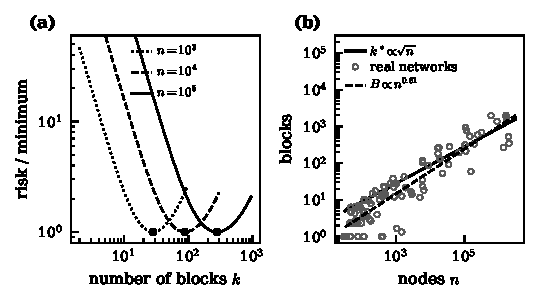
\includegraphics[width=\linewidth]{figs/fig-gr-resolution.pdf}
\caption{\textbf{How many blocks can be seen.} (a)~The risk of a $k$-block
description, Eq.~\eqref{eq:gr-risk}, for three network sizes, each normalized to
its own minimum (dots). The optimum moves right as $\sqrt{n}$. (b)~That optimum
against size, with the community counts of the real networks of the last chapter
and their fitted power law. The vertical placement of the $k^*$ line depends on
the graphon's smoothness constant and carries no meaning; its slope of one half
does.}
\label{fig:gr-resolution}
\end{figure}

And here the chapter's opening question returns, transformed. The $\sqrt{n}$ that
the last chapter used as its fractal yardstick --- the self-similar prediction of
$\sqrt{n}$ communities of $\sqrt{n}$ nodes --- turns out to be the same $\sqrt{n}$
that statistics arrives at from an entirely different direction, as the resolution
at which a smooth shape is best described. The book's models and the statisticians'
histograms agree on a number for reasons that have nothing to do with each other.

\section{Rough, not smooth}

Take the agreement seriously and the measured exponent stops being a curiosity and
becomes a measurement of something.

The real networks gave $\beta\approx0.61$, with a bootstrap interval
$[0.55,0.67]$ that excludes one half. Read through Eq.~\eqref{eq:gr-kstar}, an
exponent is no longer just a number above or below a fractal benchmark: it is a
statement about the smoothness of the shape being described. Inverting
$\beta=1/(1+\alpha)$,
\begin{equation}
  \alpha \;=\; \frac{1}{\beta}-1 \;\approx\; 0.65,
  \qquad \alpha\in[0.49,\,0.82],
  \label{eq:gr-alpha}
\end{equation}
and the interval lies wholly below $\alpha=1$. Direct minimization of
Eq.~\eqref{eq:gr-risk} at $\alpha=0.65$ returns an exponent of $0.611$, against
the measured $0.608$.

So the excess over $\sqrt{n}$ is not merely ``more communities than a fractal.''
It says that if real networks are converging to any limiting shape at all, that
shape is \emph{rough}: not Lipschitz, not smooth in the sense the estimation
theory assumes, but H\"older-continuous with an exponent around two thirds. A
smooth graphon --- any smooth graphon, of any shape, at any scale, since the
smoothness constant sets only the height of the line in
Figure~\ref{fig:gr-resolution}b and not its slope --- supports a description that
refines as $\sqrt{n}$ and no faster. Real networks refine faster than that. They
keep resolving new structure at every scale, at a rate a smooth limit cannot
supply.

This is the same conclusion the last chapter reached in its own language, and the
same one this book has been reaching since the introduction, arrived at from the
outside. A network built by a local rule has no smooth limiting shape to converge
to, because the rule keeps writing structure at whatever scale the network has
currently reached.

It is worth knowing that this is not a quarrel with the limit theory but an answer
to a question its own authors left open. Introducing a network generator built from
a singular measure rather than a function, \citet{palla2010} --- Lov\'asz among
them --- put the alternatives as plainly as they can be put:

\begin{quote}\small
Should we expect that large real graphs converge to some limiting network in a
strict sense of the convergence? Or, alternatively, their structure cannot be
mapped onto a fixed function, and only an ever-changing (with the size of the
network) measure (in the infinite network size limit becoming singular) can be used
to reflect the underlying structural complexity?
\end{quote}

\noindent That was posed in 2010 and left as a question. Equation~\eqref{eq:gr-alpha}
is a measurement bearing on it, taken across a hundred networks, and it comes down
on the second side: no fixed smooth function will do, because the description keeps
refining faster than any such function allows. The rest of this chapter is about how
far that answer can be trusted.

\section{Five meanings of one number}

A caution belongs here, and it is a sharp one. Five different arguments in this
book and its neighbouring literature all deliver $\sqrt{n}$, and they are not the
same statement:

\begin{itemize}
\item the \emph{fractal} $\sqrt{n}$ of the self-similar models --- a prediction
  about how many communities the networks themselves hold;
\item the \emph{geometric} $\sqrt{n}$ of Chapter~\ref{ch:distance} --- the
  multiplicity of shortest paths on the same lattice, a prediction about how many
  ways there are to cross it;
\item the \emph{constructive} $\sqrt{n}$ --- the resolution any cascade of equal
  cells is forced to, once its mean degree is held fixed;
\item the \emph{statistical} $\sqrt{n}$ of Eq.~\eqref{eq:gr-sqrtn} --- the best
  resolution obtainable for a smooth shape, a statement about descriptions;
\item the \emph{algorithmic} $\sqrt{n}$ --- the resolution limit of the
  non-nested block model, which cannot report more than of order $\sqrt{n}$
  groups no matter how many are present \citep{peixoto2014hier}.
\end{itemize}

The third of these is the one just met, and it is worth making explicit, because it
shows how little the number has to assume. Build a network from a singular measure
in the manner of \citet{palla2010}: divide the square into $m^2$ cells, give each a
probability, and multiply the whole pattern into itself $k$ times, so that the
picture has $m^k$ rows and grows sharper with every iteration. If the cells are all
the same size, the mean degree of the resulting network is $N m^{-2k}$, so holding
it fixed while refining the measure forces
\begin{equation}
  m^{k} \;=\; \sqrt{N/\langle k\rangle} \;\propto\; \sqrt{N} .
  \label{eq:gr-cascade}
\end{equation}
The construction resolves $\sqrt{N}$ rows because sparsity leaves it no choice. No
network, no estimator and no smoothness assumption enters that argument --- only
the bookkeeping of keeping a self-similar object sparse.

Three of the five now have reasons, and they are the same reason. The fractal and
geometric counts are a lattice's blocks and its routes tallied at the halfway point
of its own construction, and the constructive count is what any equal-celled cascade
must do to stay sparse; all three are self-similarity keeping its books. That is why
$\beta=1/2$ is the natural exponent for a self-similar object, and why measuring
$\beta>1/2$ says the object is not one --- the multifractal case, where the cells
are allowed to differ in size, has no such constraint and its exponent is free.
The remaining two agree with them for no reason at all.

The algorithmic $\sqrt{n}$ is a property of neither the network nor the ideal
description but of the instrument, and it deserves attention because the counts of
the last chapter were produced by exactly that instrument: a flat degree-corrected
block model selected by description length. Its ceiling and the null hypothesis under test
have the same functional form, which is an uncomfortable coincidence.

The bias runs in the reassuring direction --- a ceiling can only suppress the
counts of the largest networks and so pull the fitted exponent \emph{down},
meaning $\beta>1/2$ is measured in spite of the instrument rather than because of
it. But the conclusion that survives is correspondingly narrower: these data
establish an exponent above one half over four decades of size, and cannot by
themselves certify that it persists asymptotically, because the estimator that
produced them is not able to report an asymptotic exponent above one half. Only
the nested block model, which lifts the ceiling to order $n/\ln n$, can settle
that, and re-running the census with it is the obvious next measurement. Should
the exponent survive, Eq.~\eqref{eq:gr-alpha} converts it directly into a
statement about the roughness of the limit.

\section{What the ring cannot tell us}

One more thing the limit view clarifies, and it is a caveat about a result rather
than a strengthening of one.

The ring of the last chapter was found to prefer being split in two, for every
range $c\ge2$. But every node of the ring is identical to every other, and the
model was explicit that there is no preferred place to cut: rotate the proposed
partition by one bead and the evidence is unchanged. In the language of limits
that is a symmetry, and a continuous one. The ring's local limit --- what an
observer sitting on a node sees, out to any fixed distance
\citep{benjamini2001} --- is an infinite line, the same in every direction, with
no communities anywhere in it.

So the ring exhibits, in the cleanest possible form, a distinction the previous
chapter's machinery does not itself draw. Evidence for splitting is not the same
as the existence of a partition to be found. The ring supplies the first without
the second: a whole continuum of cuts, all equally good, none of them recoverable
from the data, and a limit object with no structure at all. What the evidence
ratio reports is that one block is a poor description --- a true and interesting
fact --- and not that two particular blocks are the right one. For the diamond
lattice and the pseudofractal web, whose partitions are pinned by their
construction, no such degeneracy arises and the identification is sound. It is the
homogeneous case that needs the care.

The ring is also the only one of the three entitled to that local limit, and the
reason is worth recording, because it marks out exactly where this book's networks
fall. A local limit of the kind just used requires an absolute ceiling on the
degree: every node must look like every other from close up, out to a bounded
number of neighbours. The ring obliges --- every node has degree $2c$ and always
will. The diamond lattice and the pseudofractal web do not: their poles grow
without bound, reaching degree $2^t$, so no ceiling exists and the local theory
does not apply to them. Nor does the theory at the other end, which needs the
number of links to outgrow the number of nodes, while theirs stays proportional
to it.

That is a genuine gap, and the book's central examples sit in it: too heavy-tailed
for the local theory, too sparse for the global one. It is also a gap the subject
knows about and is working to close --- a recent line of work \citep{backhausz2018}
proposes treating a network not as a picture at all but as an \emph{operator}, and
recovers dense graphons and local limits as two special cases of one notion of
convergence. Whether it reaches the case that matters here --- bounded mean degree
with unbounded hubs --- is precisely the question to put to it.

\section{What clustering rules out}
\label{sec:gr-clustering}

Everything so far has been about \emph{shape} --- whether a limiting picture
exists and how finely it can be resolved. There is a blunter test, and the
introduction ran it before any of this machinery was in place.

A graphon model, of any kind, draws its links independently once the positions of
the nodes are fixed. That is what makes it tractable, and it has a consequence
that cannot be argued away: a triangle needs three links, each drawn separately,
so triangles are as rare as three coincidences. In a sparse network the clustering
coefficient of such a model collapses to the link density itself, a number of
order $\langle k\rangle/n$ --- vanishing. Real networks are not like that, and the
introduction already measured by how much. Its column $C_{\mathrm{ER}}$, computed
there as the clustering of a random network of the same size and density, is
precisely the graphon prediction:

\begin{center}
\begin{tabular}{lccc}
\hline
Network & $C$ & $C_{\mathrm{ER}}$ & $C/C_{\mathrm{ER}}$ \\
\hline
Internet (AS)          & $0.230$  & $0.00018$ & $1254$ \\
Gnutella               & $0.0055$ & $0.000076$ & $72$ \\
Yeast proteins         & $0.071$  & $0.0018$  & $39$ \\
cond-mat co-authorship & $0.657$  & $0.00026$ & $2541$ \\
\hline
\end{tabular}
\end{center}

Between forty and two and a half thousand times too many triangles. No adjustment
of the shape $W$ repairs a discrepancy of that size, because the shape is not what
is wrong: the independence is.

But the argument has to be made carefully, and the careful version is more
interesting than the crude one. The comparison above is against a \emph{constant}
graphon, and we have already seen in
Section~\ref{sec:gr-blockmodel} that the constant is the weaker of the two
baselines. Against the \emph{rank-one} graphon --- the network reshuffled to
preserve every degree --- the verdict divides. The Internet's clustering falls only
from $0.230$ to $0.123$ under that reshuffling, a factor of $1.9$: its degrees
alone, hubs and all, manufacture most of its triangles, because a node of enormous
degree is shared by many pairs and closes their triangles by accident. The
co-authorship network, whose degrees are far less extreme, still stands $356$ times
above its own reshuffling.

So the two baselines separate the systems exactly as they separated the
pseudofractal's two cuts. Where the degrees are wild, degree heterogeneity accounts
for much of the clustering and little is left to explain. Where they are tame, the
whole of it survives the strongest degree-preserving null available --- and that
residue is what Chapter~\ref{ch:friends} was written to explain. Triadic closure is
not an embellishment on a graphon; it is the thing the graphon cannot do.

\section{Locality, or exchangeability}

There is a reason all of this bears on the book's thesis rather than merely
decorating it, and it is worth ending on.

A graphon is not only a limit; it is a complete description of a certain
\emph{kind} of random network --- those whose nodes are exchangeable, meaning the
labels carry no information and any two nodes are, before we look, the same
\citep{aldous1981,diaconis2008}. Every graphon model is exchangeable and every
exchangeable model is a graphon. Exchangeability is a strong assumption, and what
it excludes is precisely geometry: a node's position, its neighbourhood, its
history. It excludes locality.

The chapters before this one have argued that networks are built by nodes acting
on what is near them --- the page a surfer reached, the friend who made the
introduction, the gene that was copied. A rule of that kind produces a network in
which position matters, in which where a node attached is written into the
structure around it. Such a network is not exchangeable, and so it has no graphon
in the ordinary sense. The failure of the limit theory to say anything useful
about real networks, which began this chapter as an inconvenience, is at bottom
the same fact this book has been documenting all along, in a different vocabulary.
Sparsity and roughness and the absence of a smooth limit are what locality looks
like when a statistician goes looking for a shape.

What the sparse limits should be instead is an open and active question, and the
theory of sparse exchangeable graphs \citep{caron2017} is one serious attempt at
it. But it would be wrong to end by filing all of this under work not yet begun,
because on one point the previous chapter has already done a piece of it without
saying so.

The companion to the $L^p$ theory \citep{borgs2018} asks what it should
\emph{mean} for a sparse network to converge, and proves that several answers that
look quite different are the same answer. One can ask that the rescaled picture
settle down. One can ask that the \emph{quotients} settle --- the tables of
block-to-block densities produced by chopping the network into parts. One can ask
that the best partition at fixed block sizes settle, or that the sum over all such
partitions, weighted, settle: a ground state energy and a free energy, in the
language of physics. These are all equivalent.

That list is the last chapter's apparatus, item by item. A quotient is exactly the
table of counts $e_{rs}$ against expectations $\Omega_{rs}$. Fixed block sizes are
exactly the candidate split. The weighted sum over labelings, with the label prior
integrated out, is exactly the evidence. And the renormalization flow
$(u_{\mathrm{in}},u_\times)\to(K,0)$ is a quotient converging --- proved by hand,
for one lattice, in precisely the sense the theorem intends. That is why the
resulting $\ln K$ per link is so indifferent to the lattice that produced it:
convergence of quotients is a statement about the limiting shape, and any
arrangement with the same limiting quotient must give the same free energy.

The hypotheses of that theorem do not cover a bounded-degree lattice, so what the
last chapter proved is not a corollary of it; the flow had to be computed. But the
agreement of the two routes is worth more than either alone, and it marks out what
a limit theory for locally grown networks would have to look like. There is also,
on the other side of Eq.~\eqref{eq:gr-alpha}, a number measured across a hundred
real networks, still waiting to be explained.

\section{A conjecture, and two questions}
\label{sec:gr-conjecture}

The chapter has so far been an audit: what the limit theories can and cannot say
about networks grown by local rules. It ends with a programme instead, because the
audit points somewhere specific.

Start from what the last chapter actually did. It took networks grown by local
rules and \emph{fitted} them --- to a stochastic block model, by Bayesian
inference. A block model is a two-variable object, a kernel
$[0,1]^2\to[0,1]$ read through group labels, and the fit was good enough to
count communities across four decades of size. So a two-variable description
already captures something real. The question is what it misses, and whether the
miss has a shape.

There is a natural guess about that shape. A local rule does not act on pairs. Triadic
closure acts on \emph{triples} --- a node, its neighbour, and that neighbour's
neighbour --- and duplication acts on a node, its copy, and their shared
neighbours, a configuration of four. If the statistics a rule generates are to be
carried by a limiting object at all, the object may need arguments enough to hold
the rule's own footprint: a kernel $[0,1]^3\to[0,1]$ where the rule closes
triangles, $[0,1]^4\to[0,1]$ where it duplicates. This suggests a conjecture.

\begin{quote}
\emph{Conjecture.} For large $n$ the limit of a locally grown network is almost
equivalent to an exchangeable object --- but one of higher order than a graphon.
The order is set by the arity of the growth rule: three for triadic closure, four
for duplication, with the fitted block model as the two-variable shadow of it.
\end{quote}

\noindent The word \emph{almost} is carrying weight, and making it precise is part
of the problem. Two questions follow, and the first is answerable now.

\subsection*{Question 1: what does the fitted block model preserve?}

Given a network grown by a local rule and the block model that Bayesian inference
fits to it, which statistics agree and which do not? The honest answer has a clean
first instalment, and the pseudofractal web supplies it, because there every
quantity is exact.

\begin{calculation}{the triangles a two-variable model can hold}
The web has $n=(3^{t+1}+3)/2$ nodes and $3^{t+1}$ links, and every node added
closes exactly one triangle, so it holds exactly $n-2$ of them. Fit chapter~6's
branch cut and ask each fitted model how many it expects, via
$\mathrm{tr}(P^3)/6$ for its expected adjacency matrix $P$.

The plain block model assigns one density per block pair. In a sparse network
those densities fall like $1/n$, and a triple of blocks contributes
$n^3\times n^{-3}$: the expected count is $O(1)$, and numerically it
\emph{saturates} at $21.3$ triangles however large the web grows. Against a true
count rising like $n$, the deficit grows like $n$ itself.

The degree-corrected model does better, and still fails. Its expected count
weights each block by its squared-degree sum $Q_r=\sum_{i\in r}k_i^2$ rather than
by its size, and for this web $Q\sim4^{t}$ while the degree sum is $S\sim3^{t}$,
so the count grows as $(Q/S)^3\sim(64/27)^t$ against a truth growing as $3^t$. The
deficit again diverges, now as
\begin{equation}
  (81/64)^{t} \;=\; n^{\,0.214}.
  \label{eq:gr-tridef}
\end{equation}
Allowing the number of blocks to grow as the data demand, $B\propto n^{\beta}$,
helps but does not close it: $B$ blocks of $n/B$ nodes contribute $O(1)$ triangles
each, hence $n^{\beta}$ in all, still short of $\Theta(n)$ by $n^{1-\beta}$.
\end{calculation}

So the answer to the first question, for this network, is sharp. A two-variable
description preserves what the cut metric sees --- block densities, degrees, the
evidence for a partition, everything the last chapter computed --- and loses the
3-point structure entirely, by a margin that widens without bound. Even a
hierarchy of blocks, refining as fast as real networks demand, recovers only
$n^{\beta}$ of the $n$ triangles.

One warning for anyone testing this at accessible sizes: the failure is not
visible early, and it changes sign. At $n\simeq3000$ the degree-corrected model
\emph{over}counts triangles fivefold, and only past $n\sim10^8$ does it cross over
to undercounting. A study stopping at ten thousand nodes would conclude the
opposite of the truth.

\subsection*{Question 2: does higher order close the gap?}

If two variables are not enough, are three? Here the conjecture meets a genuine
obstacle, and the obstacle locates exactly where its content lies.

For \emph{dense} graphs the question is already settled, and settled against the
conjecture. An exchangeable array admits the representation
$f(\xi_\emptyset,\xi_i,\xi_j,\xi_{ij})$, and for a simple dense graph the
pair-level variable $\xi_{ij}$ can always be absorbed into a threshold, leaving a
two-variable kernel. Exchangeability \emph{forces} the graphon form; no
higher-order object can add anything. Whatever the conjecture is claiming, it
cannot be claiming that.

Its content therefore lies entirely in the sparse regime --- which is the regime
this whole chapter has been about, and the reason the clustering of
Section~\ref{sec:gr-clustering} does not vanish when a graphon says it must. There,
the pair-level randomness does not wash out, and the natural object keeps
arguments indexed by \emph{pairs} rather than by nodes: not $W(x_i,x_j,x_k)$ but
something closer to $W(x_{ij},x_{ik},x_{jk})$, which is the shape the limit theory
of hypergraphs already takes. That is a refinement of the conjecture rather than a
refutation of it, and it says where to look: triadic closure makes the presence of
one link depend on two others sharing a node, and a pair-indexed kernel is the
smallest object that can express such a dependence.

\subsection*{The same failure, with the arity changed}

The diamond lattice tests whether any of this was about triangles. It cannot be:
the lattice is bipartite and contains no triangle at all. Its rule replaces each
link with two parallel paths, so the motif it manufactures is the \emph{four}-cycle,
and the same question can be put again with the arity moved by one.

\begin{calculation}{the four-cycles a two-variable model can hold}
After $t$ generations the lattice has $m=4^t$ links and $n=(2\cdot4^t+4)/3$ nodes.
Only the diamonds closed at the \emph{last} generation are still four-cycles ---
earlier ones have had their links subdivided into longer loops --- so the count is
exactly $4^{t-1}$, again proportional to $n$. Fitting chapter~6's cut into two
branches and evaluating $\mathrm{tr}(P^4)/8$:

The plain block model saturates, as before, and here the constant can be named. In
the limit the two blocks are near-independent, each of $n_r\simeq4^t/3$ nodes at
density $p\simeq9/4^{t}$, contributing $n_r^4p^4/8=81/8$ four-cycles apiece:
\begin{equation}
  \text{plain model} \;\longrightarrow\; \tfrac{81}{4} = 20.25
  \label{eq:gr-quadsat}
\end{equation}
four-cycles, for a lattice of any size.

The degree-corrected model is where the two lattices part company. Its count is
governed by the ratio of the squared-degree sum to the degree sum, and for this
lattice that ratio is not a power of $n$ at all but
\begin{equation}
  Q/S \;=\; \sum_i k_i^2 \Big/ \sum_i k_i \;=\; t+1
  \label{eq:gr-QS}
\end{equation}
exactly, so the expected four-cycle count converges to $(t+1)^4/4$: \emph{poly\-log\-arithmic}
in $n$, against a truth growing as $n/6$. At $t=26$ the lattice holds
$1.1\times10^{15}$ four-cycles and the fitted degree-corrected model expects
$1.3\times10^{5}$ of them.
\end{calculation}

That gap --- a factor of $n/(\ln n)^4$ --- is far worse than the pseudofractal's
$n^{0.214}$, and the reason is the one thing the two lattices genuinely differ in.
The pseudofractal's degrees are wild, $\gamma\simeq2.585$, and a rank-one model
with hubs that extreme manufactures a great many triangles by accident: three
links that all happen to touch the same few enormous nodes close a triangle
whether or not any rule intended it. The diamond's degrees are milder,
$\gamma=3$ exactly, which is the marginal case where $\sum k_i^2$ outgrows
$\sum k_i$ only logarithmically --- and a rank-one model then has nothing to fake
with.

So the two-variable model's apparent grasp of higher-order structure is not a grasp
at all. It is borrowed entirely from degree heterogeneity, and it fails as the
degrees become tame. That is a mechanism for something already measured in
Section~\ref{sec:gr-clustering}: there the degree-preserving null came within a
factor of $1.9$ of the Internet's clustering, whose degrees are extreme, and fell
$356$ times short for co-authorship, whose degrees are not. The deterministic
lattices say why, and warn against the natural misreading --- that degree-corrected
models capture clustering. They capture it exactly where the degrees are heavy
enough to counterfeit it.

\subsection*{The whole spectrum at once}

Triangles and four-cycles are two points. Asking the question at every cycle
length turns the finding from a shortfall into something more damaging.

\begin{calculation}{why a two-variable model has a one-parameter spectrum}
For a model with independent links and expected adjacency $P$, the expected number
of $L$-cycles is $\mathrm{tr}(P^L)/2L$. When $P$ is a $K$-block fit this collapses
onto a $K\times K$ \emph{transfer matrix}
\begin{equation}
  T_{rs} \;=\; \omega_{rs}\sqrt{Q_rQ_s}
  \qquad\text{(degree-corrected)},
  \label{eq:gr-transfer}
\end{equation}
with $Q_r=\sum_{i\in r}k_i^2$, and $T_{rs}=p_{rs}\sqrt{n_rn_s}$ for the plain
model, so that the count at every length is $\mathrm{tr}(T^L)/2L$. The entire motif
spectrum is generated by one small matrix, and for large $L$ it is
$\lambda^L/2L$ for the leading eigenvalue $\lambda$ --- a smooth geometric profile.
A two-variable model has no freedom to put a feature at one particular length,
whatever its blocks are doing.
\end{calculation}

The lattices do nothing but put features at particular lengths. The diamond is
built from four-cycles and carries cycles of length $4$, $8$, $16$, and so on ---
and \emph{exactly none} at any other length. Counted directly at $t=5$: zero
$3$-cycles, $256$ four-cycles, zero at five, six and seven, $1024$ eight-cycles.
The fitted models, meanwhile, expect $8.3$ triangles, $42$ five-cycles and $104$
six-cycles under the plain fit, and $69$, $1560$ and $8171$ under the
degree-corrected one, at lengths where the lattice contains nothing whatever.

So the failure is not that the numbers are too small. It is that a two-variable
model places mass at every length while a locally grown lattice places it at a
few, and no adjustment of blocks or degrees can move a smooth profile onto a
sparse set of lengths. This is a stronger statement than the triangle deficit, and
it is the one that argues for the conjecture: what a higher-order object buys is
not a bigger number but the ability to have a shape.

The pseudofractal makes the same point from the other side. Its degree-corrected
fit does not merely undercount; it \emph{changes sign} along the spectrum,
running short at $L=3$ and then overshooting ever more wildly --- by a factor of
$20$ at $L=5$ and $10^4$ at $L=8$. The reason is now visible in
Eq.~\eqref{eq:gr-transfer}: the leading eigenvalue of a degree-corrected fit is
essentially $\langle k^2\rangle/\langle k\rangle$, so its spectrum grows like
that ratio raised to the length, and for a degree distribution $p(k)\sim
k^{-\gamma}$,
\begin{equation}
  \lambda \;\sim\; n^{(3-\gamma)/(\gamma-1)} \quad (\gamma<3), \qquad
  \lambda \sim \ln n \quad (\gamma=3).
  \label{eq:gr-lambda}
\end{equation}
For the pseudofractal, $\gamma\simeq2.585$ gives the exponent $0.2619$, which is
exactly the growth its transfer matrix shows; for the diamond, $\gamma=3$ gives
the logarithm and $Q/S=t+1$. One quantity therefore governs both earlier results:
the deficit at length $L$ is of order $n/\lambda^{L}$, undercounting while
$\lambda^L<n$ and overcounting after. The rank-one part does not describe
higher-order structure at any length. It manufactures a geometric series and
happens to cross the truth once.

Two things would move this further. On the deterministic side the crossing point
is a prediction to test: Eq.~\eqref{eq:gr-lambda} says it sits at
$L^\ast=(\gamma-1)/(3-\gamma)$, which is near $4$ for the pseudofractal and
recedes to infinity as $\gamma\to3$. On the real networks the deficit is
measurable directly --- fit the block model, sample from the fit, and compare motif
counts with the original. If the conjecture holds, the gap should close as the
order of the fitted object rises to the arity of the rule that built the network,
and stop closing thereafter.
